\subsection{Wizja dziedziny}
System klasy DMS (Dealer Management System) ma za zadanie stanowić centralny, zintegrowany system informatyczny nowoczesnego salonu samochodowego. Główną propozycją wartości biznesowej jest stworzenie środowiska, które przeprowadzi pojazd oraz klienta przez pełen cykl życia – od pierwszego zapytania ofertowego i wyboru konfiguracji (kontekst główny: Sprzedaż i CRM), poprzez logistykę dostawy, proces sprzedaży, aż po finansowanie i rozliczenie.

Nadrzędnym celem architektonicznym i biznesowym systemu jest wyeliminowanie rozproszenia danych oraz zapewnienie pojedynczego źródła prawdy (ang. \textit{Single Source of Truth}) dla każdego etapu realizowanego procesu. System automatyzuje powtarzalne procesy operacyjne, redukuje błędy ludzkie oraz zabezpiecza interesy finansowe salonu samochodowego.

Zgodnie z naturą modelu dziedziny, na całościową wizję systemu składają się następujące komponenty, uszczegółowione w kolejnych sekcjach niniejszego dokumentu:

Wymagania funkcjonalne i niefunkcjonalne są skupione wokół wartości biznesowych takich jak spójność danych, identyfikowalność pojazdów oraz zgodność prawno-finansowa.

Scenariusze przypadków użycia odzwierciedlające kluczowe procesy biznesowe (w tym proces konfiguracji, weryfikacji finansowania oraz wydania pojazdu) zostały opisane w ramach poszczególnych kontekstów.

Wizualizujące granice modeli oraz relacje strategiczne między zespołami zostały przedstawione na diagramie Context Map (sekcja 2.4) oraz Bounded Context Canvas.

\subsection{Określenie dziedziny i poddziedzin}

Główną dziedziną systemu jest zintegrowane zarządzanie nowoczesnym salonem samochodowym. Zgodnie z rygorystycznym podejściem metodyki \textit{Domain-Driven Design}, całkowity obszar działalności biznesowej został podzielony na mniejsze poddziedziny w stosunku 1:1 do planowanych kontekstów ograniczonych. Pozwala to precyzyjnie zidentyfikować obszary, w których salon generuje unikalną przewagę konkurencyjną, oraz te, które są standardowymi procesami rynkowymi.

Zidentyfikowano następujące pięć poddziedzin:

\begin{itemize}
    \item \textbf{Sprzedaż i obsługa klienta}\\
    Stanowi fundament strategiczny systemu, bezpośrednio determinujący wartość biznesową przedsiębiorstwa. Obejmuje unikalną logikę procesów ofertowych, negocjacji, budowania relacji z nabywcą oraz zarządzanie pełnym cyklem życia zamówienia.

    \item \textbf{Zarządzanie asortymentem i specyfikacją}\\
    Obszar biznesowy odpowiedzialny za parametryzację oferty pojazdów. Obejmuje pilnowanie poprawności technologicznej samochodów, weryfikację reguł wykluczeń producenta oraz dostarczanie aktualnych cenników bazowych dla procesu sprzedaży.

    \item \textbf{Gospodarka magazynowa i logistyka}\\
    Poddziedzina odpowiedzialna za fizyczne zarządzanie zasobami (placem salonu samochodowego) oraz przepływem pojazdów. Do głównych zadań należy monitorowanie statusów logistycznych aut oraz zarządzanie numerami VIN.

    \item \textbf{Pośrednictwo finansowe}\\
    Obszar wspierający sprzedaż poprzez zewnętrzną weryfikację zdolności kredytowej i leasingowej klientów. Wymaga izolowanej komunikacji z instytucjami bankowymi, co z punktu widzenia inżynierii opiera się na powtarzalnych wzorcach integracyjnych.

    \item \textbf{Księgowość i rozliczenia transakcji}\\
    Obszar obejmujący obsługę fakturowania, ewidencję zadatków oraz procesy księgowe. Dziedzina ta charakteryzuje się najwyższym stopniem unifikacji, opartym na przepisach prawa i standardach rachunkowości, niezależnym od specyfiki samego salonu samochodowego.
\end{itemize}

\begin{figure}[H]
    \centering
    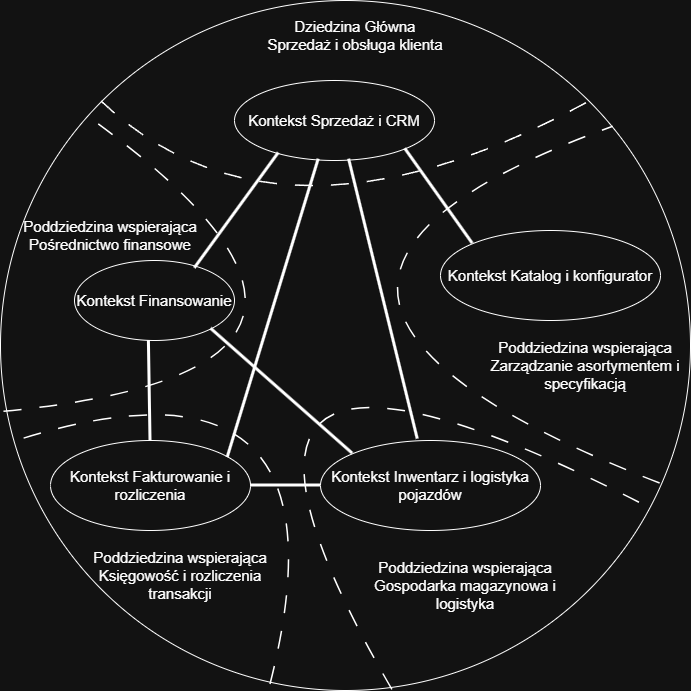
\includegraphics[width=\textwidth]{media/diagramy/mapa-kontekstow-final.png}
    \caption{Mapa kontekstów}
    \label{fig:hex_billing}
\end{figure}

\subsection{Konteksty ograniczone}

Aby zapobiec tworzeniu tzw. \textit{Big Ball of Mud} i umożliwić niezależny rozwój systemu, zdefiniowane wyżej poddziedziny biznesowe zostały odwzorowane w pięć kontekstów ograniczonych (obszarów rozwiązania IT). Granice każdego z nich wyznaczają zamknięty zakres obowiązywania języka wszechobecnego.

\begin{table}[H]
\centering
\small
\renewcommand{\arraystretch}{1.3}

\begin{tabular}{|p{3.2cm}|p{2cm}|p{3.5cm}|p{5.3cm}|}
\hline

\textbf{Poddziedzina} &
\textbf{Typ} &
\textbf{Kontekst Ograniczony} &
\textbf{Uzasadnienie}
\\
\hline

Sprzedaż i obsługa klienta &
Główna &
Sprzedaż i CRM &
Kontekst obejmuje relację z klientem, logikę ofertowania oraz cykl życia zamówienia.
\\
\hline

Zarządzanie asortymentem i specyfikacją &
Wspierająca &
Katalog i konfigurator &
Kontekst odpowiada za poprawność technologiczną specyfikacji, reguł wykluczeń oraz dystrybucję cenników.
\\
\hline

Gospodarka magazynowa i logistyka &
Wspierająca &
Inwentarz i logistyka pojazdów &
Kontekst odpowiada za fizyczne zarządzanie pojazdami na placu oraz śledzenie numerów VIN.
\\
\hline

Pośrednictwo finansowe &
Wspierająca &
Finansowanie &
Integracja z zewnętrznymi interfejsami (systemy bankowe oraz leasingodawców) realizowana przez bezpieczny wzorzec ACL.
\\
\hline

Księgowość i rozliczenia transakcji &
Wspierająca &
Fakturowanie i rozliczenia &
Obsługa dokumentów skarbowych (faktury VAT) oraz bezpieczna ewidencja wpłat i zadatków.
\\
\hline

\end{tabular}

\caption{Bezpośrednie mapowanie poddziedzin na konteksty ograniczone}
\label{tab:ddd_mapping}

\end{table}